% Model framework - similar to materials and methods, but with more paragraph
% continuity

\subsection*{Framework conception and configuration}

The proposed framework for prediction of protein-protein interactions


\subsection*{Framework evaluation on the human interactome}

As the first step in the evaluation of A2, A3 and L3 methods for link
prediction, the full calculation and ranking of all predictions was
carried out. The results for the analyzed human interactomes (\emph{HI-II-14}
and \emph{HI-TESTED}) is shown in Figure \ref{fig:HI1}, in which
the x axis represents a rank position $k$ and the y axis displays
the precision for the top $k$ predictions of each method, when assuming
interactome \emph{HI-III} as the validation set. 
	
\begin{figure}[h]
\caption{\label{fig:HI1}Methods Comparison for \emph{HI-II-14} and \emph{HI-TESTED}}
	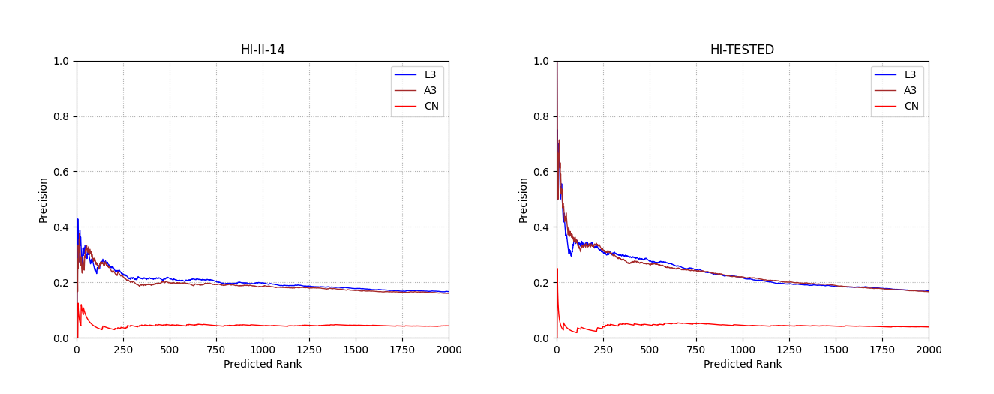
\includegraphics[width=\textwidth ]{figures/figure2.eps}
	%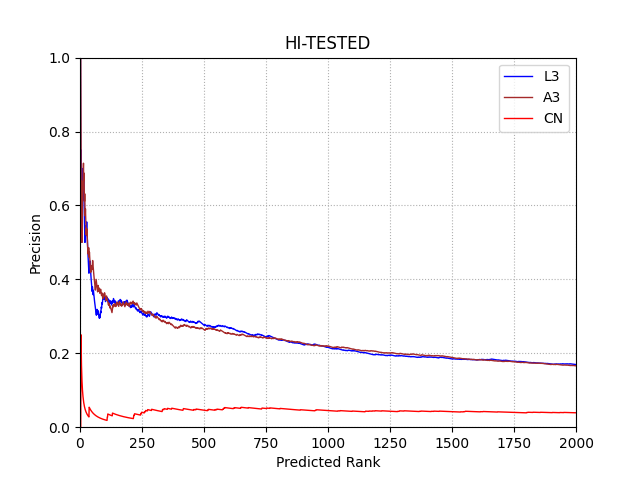
\includegraphics[width=0.7\textwidth ]{../hi-tested.txt.}
\end{figure}

As it can be inferred from the plots, L3-based predictions outperform
their $A{{}^2}$ counterparts. Results also show that L3-score and
$A^{3}$predictions follow a very similar trend.

However, it is of our interest to assess if Machine Learning can boost
the overall performance on the prediction, so the proposed procedure
was adapted to the human interactome data: Instead of having to remove
a fraction of edges from the network in order to predict and validate,
the prediction network and the validation networks are given beforehand.
The rest of the procedure is carried out as mentioned in Section 2.
Table \ref{T1} presents the results for the combinations of Node2Vec
with each feature.

\begin{table}
\caption{\label{T1}Summary statistics for human interactomes}
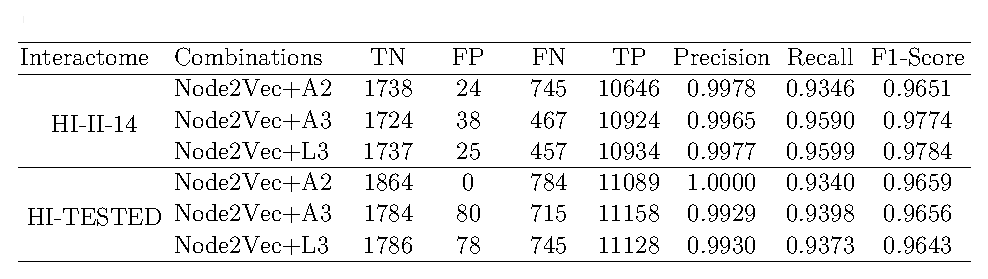
\includegraphics[width=1\columnwidth]{figures/T1}
\end{table}

In general, performance of all models is above 0.96 in terms of F1-Score.
Although marginally, the A2 feature-enriched model for HI-TESTED performs
better than their counterparts based on paths of length 3. The opposite
is also true for HI-II-14: models enriched with L3 and A3 features
perform better than their A2 counterpart. Results for the Interactome
\emph{HI-II-14} with Node2Vec and each metric are presented in Figures
S\ref{HI1}, S\ref{HI2} and S\ref{HI3}. It can be seen that for
\emph{HI-II-14}, A2 performs marginally better than L3 when comparing
precision but worse in terms of recall, although all metrics have
AUC values of 0.99.

On the other hand, the interactome \emph{HI-TESTED} was assessed with
the same methodology as \emph{HI-II-14} and results are shown in Figures
S\ref{HI1-1}, S\ref{HI2-1} and S\ref{HI3-1}. For this interactome,
A2 performs better in terms of false positives than A3 and L3, but
in terms of false negatives, A3 actually performs better that A2 and
L3. In terms of AUC, metrics results are indistinguishable. 

An interesting assessment from this human datasets can be observed
when looking at the importance plots, which show a very biased influence
of the handcrafted features. Figure \ref{F8-importance-H1} shows
this behavior for the \emph{HI-II-14} dataset, which is very similar
to \emph{HI-TESTED} (Figure S\ref{F8-importance-H2}).

\begin{figure}[h]
\noindent \begin{centering}
\caption{\label{F8-importance-H1}Importance gain plots for \emph{HI-II-14}}
\par\end{centering}
\begin{centering}
\includegraphics[width=0.48\columnwidth]{figures/Human/Imp\lyxdot A2\lyxdot 1\lyxdot eps}\includegraphics[width=0.48\columnwidth]{figures/Human/Imp\lyxdot A3\lyxdot 1\lyxdot eps}
\par\end{centering}
\centering{}\includegraphics[width=0.48\columnwidth]{figures/Human/Imp\lyxdot L3\lyxdot 1}
\end{figure}